\chapter{Linies de transmissió carregades}

\section{Introducció}

Fins ara les línies eren infinites, però necessàriament ha d' haver un generador al principi i un dispositiu al final que reba les ones: equips de mesura, antenes, filtres, forns de microones... Aquestes discontinuïtats, anomenades càrregues, no donen problemes a freqüències baixes, però a altes poden provocar reflexions, pel que tindrem dues ones en la guia. En el circuit les representarem com a impedàncies (figura \cref{circeq})  En aquesta secció anomenarem $z=0$ al punt on la guia es connecta a la càrrega.
\begin{figure}[ht]
  \centering
  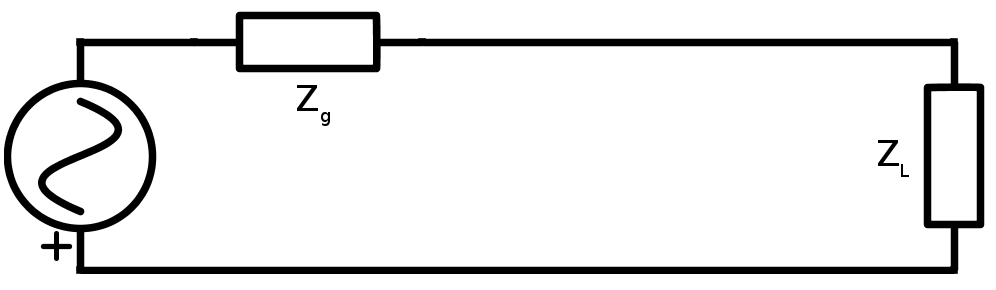
\includegraphics[scale=0.20]{circ0}
  \caption{Circuit equivalent a una guia carregada i amb generador}
  \label{circeq}
  \vspace{-2 em}
\end{figure}

\section{Coeficient de reflexió en la càrrega}

La impedància de la càrrega (vore figura \cref{genplusload})
\begin{equation}
  Z_L = \frac{V_L}{I_L} = \frac{V_0 ^+ + V_0 ^-}{I_0 ^+ + I_0 ^-}
\end{equation}
 está relacionada amb la de la ona
\begin{equation}
  Z_C = \frac{V_0 ^+}{I_0^+} = - \frac{V_0 ^-}{I_0 ^-}
\end{equation}
per el coeficient de reflexió $\Gamma = \frac{V_0 ^-}{V_0 ^+}$ seguint la relació $\Gamma = \frac{Z_L - Z_C}{Z_L + Z_C}$, pel que la fracció d' energia reflectida dependrà de la diferència entre $Z_L$ i $Z_C$. Com que mesurar impedàncies és complicat és preferible usar el $\Gamma $ per a estudiar els efectes de les càrregues.
\begin{figure}[ht]
  \centering
  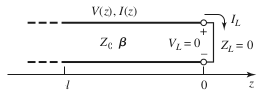
\includegraphics[scale=0.7]{loadint}
  \caption{Intensitat i voltatge en la càrrega}
  \label{genplusload}
\end{figure}

Observem que en un circuit obert, en que $Z_L = \infty$, tota l' ona és reflectida ($\Gamma = 1$) i en un curtcircuit, on $Z_L = 0$, la ona es reflexa canviada de fase ($\Gamma = -1$). En el cas en que la càrrega està adaptada a la guia $Z_L = Z_C$ tenim que $\Gamma = 0$, i és el cas òptim en que no existeixen reflexions. És per això que quasi totes les guies i dispositius tenen una impedància de $50 \Omega$.

\section{Potència consumida}

De la expressió per a la potència consumida per una resistència podem obtindre la potència consumida per la càrrega:
\begin{equation}
 \begin{split}
    P_L =& \frac{1}{2} \Re (V_L \cdot I_L ^*) = \frac{1}{2} \Re \left [ (\vp + \vm)(\ip + \im) \right]  \nonumber \\
  = &\frac{1}{2} \Re \left [ \vp (1+\Gamma _L) \left ( \frac{\vp}{Z_L} \right ) ^ * (1- \Gamma _L) \right] \nonumber \\
  = &\frac{1}{2} \abs \vp \Re \left [ \frac{1}{Z_C ^*}(1 - \abs{ \Gamma_L } ^2 + 2)\abs {\Gamma _L} ^2\sin \theta) \right]
  \end{split}
\end{equation}

Si $Z_C \in \Re$, com és el cas quan la guia té poques pèrdues, la podem deixar
\begin{equation}
  \label{eq:pot}
  P = \frac{1}{2} \frac{\abs \vp ^2}{Z_C} (1 - \abs {\Gamma_L} ^2)
\end{equation}

En aquesta expressió el primer terme és la potència que l' ona incident du cap endavant, mentre que el segon ens diu quin percentatge d' aquesta no és consumit per la càrrega.

\section{Ones estacionàries}

Quan dos ones viatjant en direccions oposades es superposen obtenim una ona estacionària:
\begin{subequations}
  \begin{align}
    V(z) = \vp \e{- \jmath \beta z} + \vm \e{ \jmath \beta z} \\
    I(z) = \ip \e{- \jmath \beta z} + \im \e{ \jmath \beta z}
  \end{align}
\end{subequations}

Per conveniència i conveni definim $\l = -z $, i reescrivim aquestes expressions com
\begin{subequations}
  \begin{align}
    V(\l) & = \vp \e{- \jmath \beta z} (1 + \Gamma _L \e{-\jmath 2 \beta z}) \nonumber \\
         & = \vp \e{ \jmath \beta \l} (1 + \abs {\Gamma _L} \e{\jmath (2 \beta \l + \theta)}) \\
    I(\l) &= \frac{\vp}{Z_L} \e{ -\jmath \beta z} (1 - \Gamma _L \e{-\jmath 2 \beta z}) \nonumber \\
\label{guideI}
         &= \frac{\vp}{Z_L} \e{ \jmath \beta \l} (1 - \abs{\Gamma _L} \e{\jmath (2 \beta \l + \theta)}) 
  \end{align}
\end{subequations}

\section{Impedància d' entrada d' una línia}

Així com en el punt $z = 0$ (el punt de la càrrega) hem definit $Z_L$ i $\Gamma _L$  a partir de $\vp$, $\vm$, ... podem fer el mateix en qualsevol punt de la línia, i definir del quocient de reflexió d' entrada entre les dues ones:
\begin{equation}
  \Gamma _{in} = \frac{V_z ^- }{V_z ^ +} = \frac{\vm \e{\jmath \beta z}}{\vp \e{-\jmath \beta z}} = \Gamma _L \e{\jmath 2 \beta z} = \abs { \Gamma _L } \e{- \jmath (\theta -2 \beta \l)}
\end{equation}

Continuant l' analogia podem definir la impedància d' entrada de la línia com el quocient
\begin{equation}
  Z_L = \frac{V(z)}{I(z)} = \frac{V^+ (z) + V^-(z)}{I^+(z) + I^- (z)} = Z_C \frac{V^+ (z) + V^-(z)}{V^+(z) - V^- (z)} = Z_C \frac{1+ \Gamma _{in}}{1 - \Gamma _{in}}
\end{equation}

La impedància d' entrada de la línia pot ser reescrita usant solament les propietats de la línia:
\begin{equation}
  Z_{in} = Z_C \frac{Z_L + Z_C \jmath \tan (\beta \l)}{Z_C + Z_L \jmath \tan (\beta \l)}
\end{equation}

La impedància puntual és per tant periòdica en $\frac{\lambda}{2}$, i quan $\beta \l = n\frac{\lambda}{2}$ és com si no hi haguera línia entre el punt $z$ i la càrrega $ Z_{in} = Z_L$, com en la figura \cref{imptoimp}.

\begin{figure}[ht]
  \centering
  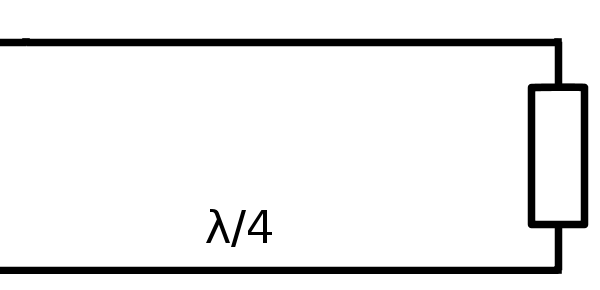
\includegraphics[scale=0.35]{impllarg}
  \quad
  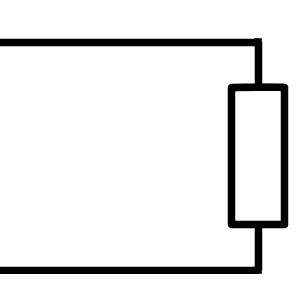
\includegraphics[scale=0.35]{impcurt}
  \caption{Impedàncies equivalents}
  \label{imptoimp}
\end{figure}

 Quan la línia és d' un quart d' ona, o $\l =  = \frac{\lambda}{4} + n \frac{\lambda}{2}$, el terme $\tan (\beta \l)$ es dispara a $\infty$, i la impedància és
\begin{equation}
  Z_{in} =  \frac{Z_C ^2}{Z_L}
\end{equation}

Una línia així s' anomena transformador de quart d' ona, perquè pot transformar la càrrega de diverses maneres. Si la càrrega és una inductància de valor $L$, la impedància en el punt $l$ serà igual a la d' un capacitador (vore figura \cref{indtocond}).
\begin{equation}
  Z_{in} = \frac{Z_C ^2}{jL\omega} = Z_{condensador}
\end{equation}

\begin{figure}[ht]
  \centering
  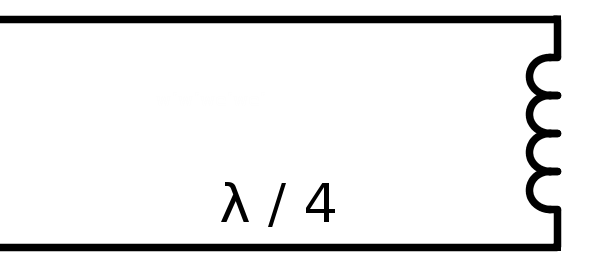
\includegraphics[scale=0.3]{inducllarg}
  \quad
  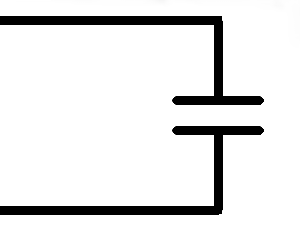
\includegraphics[scale=0.35]{condcurt}
  \caption{L' inductància i el transformador donen lloc a un capacitador}
  \label{indtocond}
\end{figure}

I si la càrrega és un capacitador, la impedància serà la d' una inductància (figura \cref{condtoind}) tindrem
\begin{equation}
  Z_{in} = j C \omega Z_C^2 = Z_{inductor}
\end{equation}

\begin{figure}[ht]
  \centering
  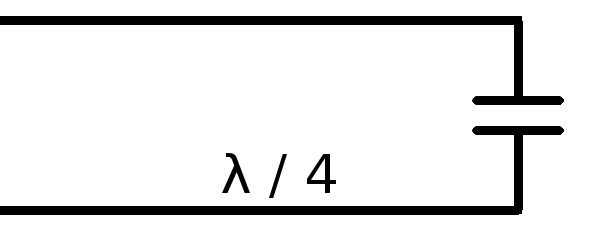
\includegraphics[scale=0.35]{condllarg}
  \quad
  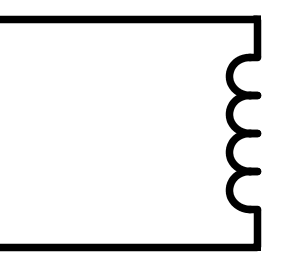
\includegraphics[scale=0.3]{induccurt}
  \caption{El condensador i el transformador donen lloc a un inductor}
  \label{condtoind}
\end{figure}

Com els inductors ''de llibre'' són difícils de construir podem utilitzar aquest resultat per a construir-los usant un condensador amb una guia de quart d' ona.

\section{Generador i línia}

Tots els anàlisis fets fins ara estan en funció de $\vp$, que depén del generador que alimenta la línia. Aquest està caracteritzat per tres variables: $V_g$, $\omega$ i $Z_g$. Relacionar $V_g$ i $V_0$, però, és complicat.

La càrrega i el segment de línia entre el generador i aquesta poden ser estudiats com una sola impedància (vore figura \cref{circeq})  per la que passa una corrent
\begin{equation}
  I_L = \frac{V_g}{Z_g + Z_{in}}
\end{equation}

Aquesta corrent ha de ser igual a la que corre per la guia \cref{guideI}, i igualant-les obtenim la relació entre els voltatges:
\begin{equation}
  I_L = I(l) \to \frac{V_g}{Z_g + Z_{in}} = \frac{\vp}{Z_C} \e{\jmath \beta \l} (1 - \Gamma _{in})
\end{equation}

I per tant
\begin{equation}
  \vp = V_g \e{- \jmath \beta \l} \frac{Z_C}{Z_g + Z_C + \Gamma _{in}(Z_C - Z_g)}
\end{equation}
pel que $\abs \vp = f(V_g, \l)$ i tenim el problema de que la potència consumida dependrà de la distància ( a través de $\Gamma_{in}$), el que seria inconvenient perquè ens obligaria a usar guies que foren múltiples d' una certa distància o perdre energia. El significat físic d' açò és que la ona torna a reflectir-se en el generador, i perdem energia.

Aquest problema ve de la presència de $\Gamma _{in}$ en l' expressió que relaciona $\vp$ i $V_g$. Una solució simple és assegurar-se de que $Z_C = Z_g$, i així
\begin{equation}
  \abs \vp = Z_C \frac{V_g \e{- \jmath \beta \l }}{Z_g + Z_C}
\end{equation}

Per conveni els generadors es fabriquen quasi sempre de manera que la $Z_g$ siga de 50 $\Omega$, igual que les guies. El desavantatge és que la impedància interior del generador consumirà energia, però és preferible.